\documentclass[11pt,letterpaper]{article}

% --- Idioma y formato -------------------------------------------------------
\usepackage[T1]{fontenc}
\usepackage{lmodern}
\usepackage[spanish,es-tabla,es-nodecimaldot]{babel}
\usepackage[top=3.4cm, bottom=2.3cm, left=2.3cm, right=2.3cm, headheight=60pt, headsep=0.6cm]{geometry}
\usepackage{fancyhdr}
\usepackage{graphicx}
\usepackage[table]{xcolor}
\usepackage{amsmath,amssymb}
\usepackage{siunitx}
\usepackage{booktabs,array,tabularx}
\usepackage{caption}
\usepackage{float}
\usepackage{enumitem}
\usepackage{needspace}
\usepackage{listings}
\usepackage[most]{tcolorbox}
\usepackage{tikz}
\usetikzlibrary{arrows.meta,calc,positioning,decorations.markings,babel}
\usepackage{hyperref}
\hypersetup{colorlinks=true, linkcolor=azulunal, urlcolor=azulunal}

% --- Colores ----------------------------------------------------------------
\definecolor{azulunal}{RGB}{0,82,147}
\definecolor{naranja}{RGB}{230,115,0}
\definecolor{verde}{RGB}{0,135,90}
\definecolor{gris}{RGB}{110,110,110}
\definecolor{fondocodigo}{RGB}{245,246,248}

% --- Notación (la misma de la presentación del curso) ----------------------
\newcommand{\rf}{\text{ref}}
\newcommand{\vx}{\mathbf{x}}
\newcommand{\vu}{\mathbf{u}}
\newcommand{\cod}[1]{\texttt{\detokenize{#1}}}

% --- Código Julia -----------------------------------------------------------
\lstdefinelanguage{Julia}{
  morekeywords={function,end,for,in,if,else,elseif,return,using,include,const,true,false,begin,let},
  sensitive=true, morecomment=[l]\#, morestring=[b]"}
\lstset{language=Julia, basicstyle=\ttfamily\small, keywordstyle=\color{azulunal}\bfseries,
  commentstyle=\color{gris}\itshape, stringstyle=\color{verde}, backgroundcolor=\color{fondocodigo},
  frame=single, rulecolor=\color{black!15}, framesep=4pt, xleftmargin=6pt, xrightmargin=6pt,
  columns=fullflexible, keepspaces=true, showstringspaces=false, breaklines=true,
  aboveskip=6pt, belowskip=6pt,
  literate={á}{{\'a}}1 {é}{{\'e}}1 {í}{{\'i}}1 {ó}{{\'o}}1 {ú}{{\'u}}1 {ñ}{{\~n}}1 {°}{{$^\circ$}}1}

% --- Encabezado -------------------------------------------------------------
\pagestyle{fancy}
\fancyhf{}
\fancyhead[L]{
\includegraphics[width=3cm]{Images/logo.png}}
\fancyhead[R]{\textbf{Manual rápido -- Modos de control del robot}}
\fancyfoot[C]{\thepage}

\newtcolorbox{recuadro}[1]{colback=azulunal!4, colframe=azulunal, fonttitle=\bfseries,
  title={#1}, boxrule=0.6pt, arc=2pt, left=6pt, right=6pt, top=4pt, bottom=4pt}
\newtcolorbox{ojo}{colback=naranja!6, colframe=naranja, boxrule=0.6pt, arc=2pt,
  left=6pt, right=6pt, top=3pt, bottom=3pt}

\setlist{itemsep=2pt, topsep=4pt}

% Robot visto desde arriba (adelante = +x, izquierda = +y). #1: rumbo delta en grados
% (positivo a la derecha = horario), #2: alto de la imagen.
\newcommand{\robotarriba}[3][0,0]{%
  \node[inner sep=0, rotate={-(#2)}] at (#1) {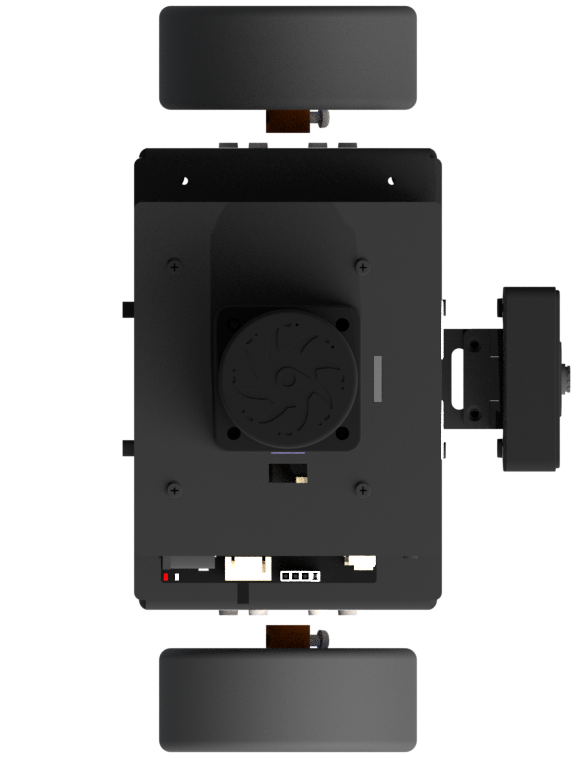
\includegraphics[height=#3]{Images/robot_arriba.png}};}

\begin{document}

% ==================== TÍTULO ====================
\begin{center}
  {\LARGE\bfseries Manual rápido: modos de control del robot}\\[4pt]
  {\large Control -- Práctica 6}\\[2pt]
  {\normalsize Universidad Nacional de Colombia -- Departamento de Ingeniería Eléctrica y Electrónica -- 2026-2}
\end{center}

\begin{minipage}[c]{0.36\textwidth}
  \centering
  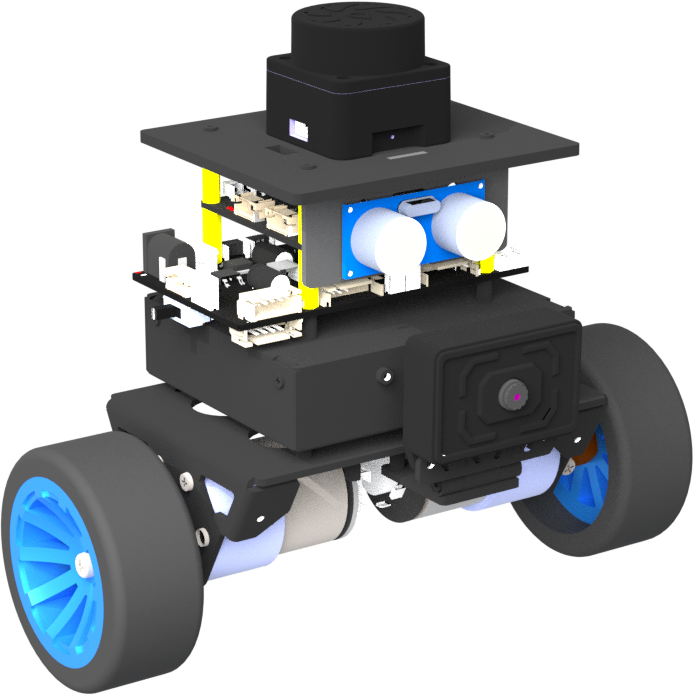
\includegraphics[width=0.92\linewidth]{Images/robot_hero.png}
\end{minipage}\hfill
\begin{minipage}[c]{0.6\textwidth}
\begin{recuadro}{Programar el robot en cuatro pasos}
\begin{enumerate}[leftmargin=*]
  \item Abra el script del modo que quiere usar, \cod{USER/control_lqr_modeN.jl}
        ($N=0,1,2,3$).
  \item Ajuste las matrices $Q$ y $R$ del diseño LQR y las referencias de la última
        línea (\cod{set_ss_controller(...)}).
  \item Conecte el robot por USB y ejecute el script con \textbf{Alt\,+\,Enter}.
        Espere el mensaje \emph{¡PROCESO COMPLETADO EXITOSAMENTE!}
  \item Ponga el robot en el piso, oprima \textbf{RESET}, espere un segundo y oprima
        \textbf{KEY1}. El robot se equilibra \textbf{5\,s en el modo 0} y luego pasa
        al modo programado.
\end{enumerate}
\end{recuadro}
\end{minipage}

\medskip
Antes de empezar, vea \href{https://www.youtube.com/watch?v=5Se6b7LLZ2M}{el video de los
cuatro modos}: muestra en simulación cómo se comporta el robot en cada uno.

% ==================== 1. VARIABLES ====================
\section{Variables y convenciones}

El firmware mide el estado cada \SI{5}{ms} (\SI{200}{Hz}) y calcula las dos entradas de
control, que son las aceleraciones de las ruedas izquierda y derecha,
$\vu=\begin{bmatrix}u_i & u_d\end{bmatrix}^{\!\top}$ en \si{m/s^2}. El estado completo es
\[
  \vx=\begin{bmatrix} x & v & \theta_c & \omega_c & \delta & \omega_\delta\end{bmatrix}^{\!\top}.
\]

\begin{figure}[H]
\centering
\begin{tikzpicture}[>=Stealth]
  % ---- (a) vista lateral ----
  \begin{scope}
    \draw[gris, thick] (-2.2,0) -- (2.6,0);
    \node[inner sep=0, anchor=south] (lado) at (0,-0.03) {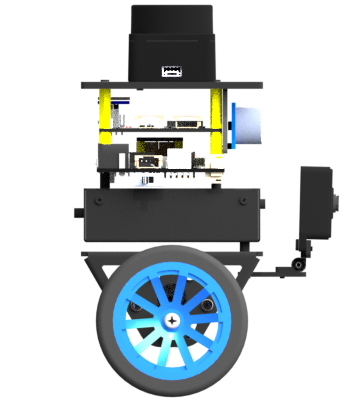
\includegraphics[height=3.4cm]{Images/robot_lado.png}};
    \coordinate (eje) at (0,0.68);
    \draw[gris, dashed] (eje) -- ++(0,3.0);
    \draw[naranja, very thick] (eje) -- ++(75:3.0);
    \draw[naranja, ->, thick] ($(eje)+(90:2.55)$) arc[start angle=90, end angle=75, radius=2.55];
    \node[naranja, above right] at ($(eje)+(84:2.6)$) {$\theta_c,\ \omega_c$};
    \draw[azulunal, ->, very thick] (1.1,-0.35) -- (2.5,-0.35) node[right] {$x,\ v$};
    \node[gris, font=\small] at (-1.5,-0.35) {adelante $\rightarrow$};
    \node[font=\small] at (0.2,-1.0) {(a) vista lateral};
  \end{scope}
  % ---- (b) vista superior ----
  \begin{scope}[xshift=7.6cm, yshift=1.6cm]
    \robotarriba[0,0]{25}{2.3cm}
    \draw[gris, dashed] (0,0) -- (2.6,0) node[right, font=\small] {$\delta=0$};
    \draw[azulunal, ->, very thick] (0,0) -- (-25:2.7);
    \draw[azulunal, ->, thick] (1.9,0) arc[start angle=0, end angle=-25, radius=1.9];
    \node[azulunal] at (-12:2.25) {$\delta$};
    \draw[naranja, ->, thick] (150:1.75) arc[start angle=150, end angle=40, radius=1.75];
    \node[naranja, above] at (95:1.75) {$\omega_\delta>0$};
    \path[rotate=-25] (0,0.95) coordinate (ri) (0,-0.95) coordinate (rd);
    \draw[gris, <-] (ri) -- ++(-1.6,0.35) node[left, font=\small, text=black] {rueda izquierda ($i$)};
    \draw[gris, <-] (rd) -- ++(-1.3,-0.55) node[left, font=\small, text=black] {rueda derecha ($d$)};
    \node[font=\small] at (0,-2.6) {(b) vista superior};
  \end{scope}
\end{tikzpicture}
\caption{Variables del robot. El giro $\delta$ es \textbf{positivo hacia la derecha}
(horario visto desde arriba): la rueda izquierda más rápida hace crecer $\delta$.}
\label{fig:variables}
\end{figure}

\begin{table}[H]
\centering\small
\begin{tabular}{@{}clll@{}}
\toprule
Símbolo & Significado & Unidad & Variable en \cod{app_control.c}\\
\midrule
$x$ & distancia recorrida (odometría de los encoders) & \si{m} & \cod{x_pose}\\
$v$ & velocidad lineal & \si{m/s} & \cod{x_speed}\\
$\theta_c$ & inclinación del cuerpo (respecto a $\theta_0=\SI{0.0349}{rad}$) & \si{rad} & \cod{angle_x}\\
$\omega_c$ & velocidad de inclinación & \si{rad/s} & \cod{gyro_x}\\
$\delta$ & giro (rumbo), positivo a la derecha & \si{rad} & \cod{angle_z}\\
$\omega_\delta$ & velocidad de giro & \si{rad/s} & \cod{gyro_z}\\
$z_v$, $z_\omega$ & integrales de los errores de $v$ y de $\omega_\delta$ & & \cod{z1}, \cod{z2}\\
$u_i$, $u_d$ & aceleración de la rueda izquierda / derecha & \si{m/s^2} & \cod{L_accel}, \cod{R_accel}\\
\bottomrule
\end{tabular}
\caption{Variables del controlador. $x$ y $\delta$ se miden desde donde estaba el robot
cuando se activó el control.}
\label{tab:variables}
\end{table}

\begin{ojo}
\textbf{Unidades.} Las referencias van en el SI, como en el firmware: metros, \si{m/s},
\textbf{radianes} y \textbf{rad/s}. Un ángulo en grados se pasa como \cod{deg2rad(45)}.
\end{ojo}

% ==================== 3. LOS CUATRO MODOS ====================
\section{Los cuatro modos}

\begin{figure}[H]
\centering
\begin{tikzpicture}[>=Stealth, font=\small]
  % ---------- Modo 0 ----------
  \begin{scope}
    \robotarriba[0,0]{0}{1.4cm}
    \draw[naranja, dashed, thick] (0.6,0) -- (3.0,0);
    \draw[naranja, thick] (3.2,0) circle (0.2); \draw[naranja] (3.0,0) -- (3.4,0) (3.2,-0.2) -- (3.2,0.2);
    \node[naranja, above] at (3.2,0.2) {$x_\rf$};
    \draw[naranja, ->, thick, dashed] (0,0) -- (-40:1.6) node[right] {$\delta_\rf$};
    \draw[naranja, ->] (1.15,0) arc[start angle=0, end angle=-40, radius=1.15];
    \node[align=center] at (1.6,-2.15) {\textbf{Modo 0}: va a $x_\rf$ con rumbo $\delta_\rf$\\ y se queda quieto};
  \end{scope}
  % ---------- Modo 1 ----------
  \begin{scope}[xshift=8.2cm]
    \robotarriba[0,0]{0}{1.4cm}
    \draw[gris, dashed] (-1.2,0) -- (4.2,0);
    \draw[naranja, ->, line width=2.2pt] (0.7,0) -- (3.0,0) node[above, pos=0.5] {$v_\rf$};
    \node[gris] at (3.6,0.3) {$\delta=\delta_\rf$};
    \node[align=center] at (1.5,-2.15) {\textbf{Modo 1}: avanza en línea recta\\ a velocidad $v_\rf$};
  \end{scope}
  % ---------- Modo 2 ----------
  \begin{scope}[yshift=-5.2cm]
    \robotarriba[0,0]{-30}{1.4cm}
    \draw[naranja, ->, very thick] (160:1.25) arc[start angle=160, end angle=-110, radius=1.25];
    \node[naranja, right] at (20:1.3) {$\omega_{\delta,\rf}>0$};
    \node[gris] at (-2.3,0) {$x=x_\rf$};
    \node[align=center] at (0.6,-2.15) {\textbf{Modo 2}: gira en el sitio\\ a velocidad $\omega_{\delta,\rf}$};
  \end{scope}
  % ---------- Modo 3 ----------
  \begin{scope}[xshift=9.4cm, yshift=-6.0cm]
    \draw[naranja, dashed, thick] (0,0) circle (1.45);
    \fill[gris] (0,0) circle (1.5pt);
    \draw[gris, <->] (0,0) -- (-140:1.45) node[midway, above left, inner sep=1pt] {$R$};
    \robotarriba[0,1.45]{0}{1.2cm}
    \draw[naranja, ->, very thick] (60:1.45) arc[start angle=60, end angle=-20, radius=1.45];
    \node[align=center] at (0,-2.25) {\textbf{Modo 3}: recorre un círculo,\\ $R=v_\rf/\omega_{\delta,\rf}$};
  \end{scope}
\end{tikzpicture}
\caption{Qué hace el robot en cada modo (vista superior). Con $\omega_{\delta,\rf}>0$ gira a la derecha.}
\label{fig:modos}
\end{figure}

\begin{table}[H]
\centering\small
\setlength{\tabcolsep}{4pt}
\begin{tabular}{@{}clll@{}}
\toprule
Modo & Controla & Orden de las columnas de $K$ ($2\times6$) & Referencias\\
\midrule
0 & posición y rumbo & $x,\ v,\ \theta_c,\ \omega_c,\ \delta,\ \omega_\delta$ & \cod{ref_pos}, \cod{ref_yaw}\\
1 & velocidad lineal & $v,\ \theta_c,\ \omega_c,\ \delta,\ \omega_\delta,\ z_v$ & \cod{ref_vel}, \cod{ref_yaw}\\
2 & velocidad de giro & $x,\ v,\ \theta_c,\ \omega_c,\ \omega_\delta,\ z_\omega$ & \cod{ref_pos}, \cod{ref_wd}\\
3 & velocidad lineal y de giro & $v,\ \theta_c,\ \omega_c,\ \omega_\delta,\ z_v,\ z_\omega$ & \cod{ref_vel}, \cod{ref_wd}\\
\bottomrule
\end{tabular}
\caption{Resumen de los modos; el script del modo $N$ es \cod{USER/control_lqr_modeN.jl}.
En todos, $K$ es de $2\times6$: fila 1 para la rueda izquierda y fila 2 para la derecha.
Los pesos de $Q$ van en el mismo orden que las columnas.}
\label{tab:modos}
\end{table}

En los modos con acción integral, el diseño en Julia aumenta el modelo reducido
$(A_r,B_r)$ con los integradores $\dot z=r-C_r\vx_r$ (referencia menos salida) y calcula
la ganancia sobre el sistema aumentado:
\[
  A_g=\begin{bmatrix}A_r & 0\\ -C_r & 0\end{bmatrix},\qquad
  B_g=\begin{bmatrix}B_r\\ 0\end{bmatrix},\qquad
  \begin{bmatrix}K & K_i\end{bmatrix}=\texttt{lqr(Continuous, Ag, Bg, Q, R)}.
\]
El modelo reducido se obtiene quitando del modelo completo el estado que no interesa
($x$ en los modos 1 y 3, $\delta$ en los modos 2 y 3). Los scripts ya traen estas matrices
construidas: basta con ajustar $Q$, $R$ y las referencias.

\subsection*{Modo 0 -- Balance con posición y rumbo}
Realimentación de los seis estados, sin integradores. Es el modo de arranque.
\[
  \vu=-K\,(\vx-\vx_\rf),\qquad \vx_\rf=\begin{bmatrix}x_\rf&0&0&0&\delta_\rf&0\end{bmatrix}^{\!\top}.
\]
\begin{lstlisting}
# Ir a 0.6 m y girar 45° a la derecha
set_ss_controller(Klqr; mode=0, ref_pos=0.6, ref_yaw=deg2rad(45))
\end{lstlisting}

\subsection*{Modo 1 -- Avance con acción integral en $v$}
No realimenta la posición. El integrador $\dot z_v=v_\rf-v$ hace que $v$ llegue a $v_\rf$
aunque haya fricción o una pendiente.
\[
  \vu=-\Big(K\begin{bmatrix}v & \theta_c & \omega_c & \delta-\delta_\rf & \omega_\delta\end{bmatrix}^{\!\top}+K_i\,z_v\Big).
\]
\begin{lstlisting}
# Avanzar a 0.2 m/s con el rumbo que tenga al terminar el arranque
set_ss_controller(Kv; mode=1, ref_vel=0.2, ref_yaw=0.0)
\end{lstlisting}

\subsection*{Modo 2 -- Giro con acción integral en $\omega_\delta$}
No realimenta el rumbo $\delta$. Mantiene la posición y el integrador
$\dot z_\omega=\omega_{\delta,\rf}-\omega_\delta$ hace que la velocidad de giro llegue
a $\omega_{\delta,\rf}$, aunque un motor sea más débil que el otro.
\[
  \vu=-\Big(K\begin{bmatrix}x-x_\rf & v & \theta_c & \omega_c & \omega_\delta-\omega_{\delta,\rf}\end{bmatrix}^{\!\top}+K_i\,z_\omega\Big).
\]
\begin{lstlisting}
# Girar en el sitio a 45°/s hacia la derecha
set_ss_controller(Kw; mode=2, ref_pos=0.0, ref_wd=deg2rad(45))
\end{lstlisting}

\subsection*{Modo 3 -- Giro y avance con acción integral en $v$ y $\omega_\delta$}
No realimenta ni la posición ni el rumbo. Los dos integradores hacen que $v=v_\rf$ y
$\omega_\delta=\omega_{\delta,\rf}$ exactamente, así que el robot recorre un círculo de
radio $R=v_\rf/\omega_{\delta,\rf}$.
\[
  \vu=-\Big(K\begin{bmatrix}v & \theta_c & \omega_c & \omega_\delta-\omega_{\delta,\rf}\end{bmatrix}^{\!\top}+K_{iv}\,z_v+K_{i\omega}\,z_\omega\Big).
\]
\begin{lstlisting}
# Círculo de radio 0.22/0.785 = 0.28 m hacia la derecha
set_ss_controller(K3; mode=3, ref_vel=0.22, ref_wd=deg2rad(45))
\end{lstlisting}

% ==================== 4. JULIA ====================
\section{Programación desde Julia}

Cada script \cod{control_lqr_modeN.jl} tiene las mismas partes: los parámetros físicos,
las matrices del modelo, la sintonía LQR ($Q$ y $R$) y, al final, la llamada a
\cod{set_ss_controller}, que hace todo lo demás (Figura~\ref{fig:flujo}).

\begin{figure}[H]
\centering
\begin{tikzpicture}[>=Stealth, font=\small,
  caja/.style={draw, rounded corners=2pt, fill=#1!8, align=center, minimum height=1.0cm, inner sep=4pt},
  caja/.default=azulunal]
  \node[caja] (jl) {\cod{control_lqr_modeN.jl}\\ $Q$, $R$ $\rightarrow$ \cod{lqr} $\rightarrow K$};
  \node[caja, right=0.7cm of jl] (set) {\cod{set_ss_controller}\\ \cod{(K; mode, refs, file)}};
  \node[caja=gris, right=0.7cm of set, align=left] (arch)
    {\cod{APP/lqr_gain_modeN.h}\\ \cod{APP/lqr_mode.h}\\ \cod{LQR.csolution.yml}};
  \node[caja=verde, below=0.8cm of arch] (cb) {\cod{cbuild}\\ $\rightarrow$ \cod{LQR.hex}};
  \node[caja=verde, left=0.7cm of cb] (fl) {\cod{stm32flash}\\ por USB};
  \node[caja=naranja, left=0.7cm of fl] (rb) {robot: RESET\\ y KEY1};
  \draw[->, thick] (jl) -- (set);
  \draw[->, thick] (set) -- (arch);
  \draw[->, thick] (arch) -- (cb);
  \draw[->, thick] (cb) -- (fl);
  \draw[->, thick] (fl) -- (rb);
\end{tikzpicture}
\caption{Qué ocurre al ejecutar un script con Alt\,+\,Enter.}
\label{fig:flujo}
\end{figure}

\begin{table}[H]
\centering\small
\begin{tabularx}{\textwidth}{@{}lllX@{}}
\toprule
Parámetro & Unidad & Por defecto & Uso\\
\midrule
\cod{K} (primer argumento) & & & matriz de ganancias de $2\times6$ (Tabla~\ref{tab:modos})\\
\cod{mode} & & \cod{0} & modo programado: 0, 1, 2 o 3\\
\cod{ref_pos} & \si{m} & \cod{0.0} & posición $x_\rf$ (modos 0 y 2)\\
\cod{ref_vel} & \si{m/s} & \cod{0.0} & velocidad $v_\rf$ (modos 1 y 3)\\
\cod{ref_yaw} & \si{rad} & \cod{0.0} & rumbo $\delta_\rf$ (modos 0 y 1), positivo a la derecha\\
\cod{ref_wd} & \si{rad/s} & \cod{0.0} & velocidad de giro $\omega_{\delta,\rf}$ (modos 2 y 3), positiva a la derecha\\
\cod{file} & & \cod{"app_control.c"} & archivo C del controlador (Sección~\ref{sec:archivo})\\
\bottomrule
\end{tabularx}
\caption{Parámetros de \cod{set_ss_controller}.}
\label{tab:parametros}
\end{table}

Al ejecutarse, \cod{set_ss_controller}:
\begin{enumerate}
  \item Comprueba que $K$ sea de $2\times6$ y escribe en \cod{APP/} las ganancias del modo
        (\cod{lqr_gain_modeN.h}) y el modo con todas las referencias (\cod{lqr_mode.h}).
        Los headers de los otros modos no cambian: el firmware compila las ganancias de los
        cuatro, con las últimas que se programaron para cada uno.
  \item Escribe en \cod{USER/LQR.csolution.yml} qué archivo C se compila como controlador.
  \item Busca el puerto USB del robot, compila el firmware con \cod{cbuild} (Arm Keil Studio /
        CMSIS-Toolbox) y graba el \cod{.hex} con \cod{stm32flash}. El robot entra solo en
        modo de grabación: no hace falta oprimir botones durante la grabación.
\end{enumerate}

\begin{ojo}
\textbf{Consejos de sintonía.} Parta de los valores de $Q$ y $R$ que traen los scripts y
cambie un peso a la vez. Un peso mayor en $Q$ hace que ese estado se corrija más rápido
y gasta más esfuerzo de los motores; un peso mayor en $R$ hace el control más suave. En el
modo 2, pesos muy grandes en $\omega_\delta$ pueden hacer oscilar el giro en el robot real
aunque el diseño continuo sea estable.
\end{ojo}

% ==================== 5. ARCHIVO PROPIO ====================
\needspace{9\baselineskip}
\section{Usar su propio archivo de controlador}
\label{sec:archivo}

El lazo de control está en \cod{APP/app_control.c}. Para probar una ley de control propia
sin modificar ese archivo:
\begin{enumerate}
  \item Copie \cod{APP/app_control.c} con otro nombre, por ejemplo \cod{APP/mi_control.c},
        y haga los cambios en la copia.
  \item Pase el nombre en la llamada:\nopagebreak
\begin{lstlisting}[nolol]
set_ss_controller(Klqr; mode=0, ref_pos=0.0, file="mi_control.c")
\end{lstlisting}
\end{enumerate}
El archivo se busca en \cod{APP/}, luego en \cod{USER/} y luego en el directorio actual;
también se acepta una ruta absoluta. Debe definir lo mismo que \cod{app_control.c}, porque
el resto del firmware lo usa: la interrupción \cod{EXTI15_10_IRQHandler} (el lazo de
control), las funciones \cod{Get_Angle}, \cod{Set_Control_Mode} y \cod{Get_Control_Mode},
y las variables globales \cod{battery} y \cod{Flag_velocity}. El último archivo usado queda
anotado en \cod{LQR.csolution.yml}; para volver al original, ejecute un script sin
\cod{file}. Keil µVision (\cod{LQR.uvprojx}) compila siempre \cod{app_control.c}.

% ==================== 6. PROBLEMAS ====================
\section{Problemas frecuentes}

\begin{table}[H]
\centering\small
\begin{tabularx}{\textwidth}{@{}>{\raggedright\arraybackslash}p{6.3cm}X@{}}
\toprule
Mensaje o síntoma & Qué hacer\\
\midrule
\emph{No se encontró ningún puerto USB-serial compatible} & Conecte el cable USB al robot
  y enciéndalo.\\
\emph{Se encontraron múltiples puertos candidatos} & Desconecte los otros dispositivos
  USB-serial (otra tarjeta, un ESP32, \dots).\\
\emph{En el modo N la matriz K debe ser 2×6} & Revise que el sistema aumentado tenga seis
  estados y que pase la $K$ del modo correcto.\\
\emph{No se encontró el archivo del controlador} & Revise el nombre que pasó en \cod{file}
  y que el archivo esté en \cod{APP/} (o pase la ruta completa).\\
Advertencia: \emph{ref\_yaw \dots\ es más de una vuelta} & Pasó grados: use
  \cod{deg2rad(...)}.\\
\emph{No se localizaron: cbuild, cmake, \dots} & Abra el proyecto en VS Code con Arm Keil
  Studio para que instale las herramientas de compilación.\\
El robot no arranca después de grabar & Oprima RESET, espere un segundo y oprima KEY1. Con
  la batería por debajo de \SI{9.6}{V} los motores no se encienden.\\
El robot se cae o se desvía al cambiar de modo & Revise los pesos de $Q$ y $R$ del modo
  programado: a los \SI{5}{s} empieza a usar sus ganancias.\\
\bottomrule
\end{tabularx}
\caption{Errores frecuentes al programar el robot.}
\end{table}

\end{document}
